\documentclass[twoside]{book}

% Packages required by doxygen
\usepackage{fixltx2e}
\usepackage{calc}
\usepackage{doxygen}
\usepackage[export]{adjustbox} % also loads graphicx
\usepackage{graphicx}
\usepackage[utf8]{inputenc}
\usepackage{makeidx}
\usepackage{multicol}
\usepackage{multirow}
\PassOptionsToPackage{warn}{textcomp}
\usepackage{textcomp}
\usepackage[nointegrals]{wasysym}
\usepackage[table]{xcolor}

% Font selection
\usepackage[T1]{fontenc}
\usepackage[scaled=.90]{helvet}
\usepackage{courier}
\usepackage{amssymb}
\usepackage{sectsty}
\renewcommand{\familydefault}{\sfdefault}
\allsectionsfont{%
  \fontseries{bc}\selectfont%
  \color{darkgray}%
}
\renewcommand{\DoxyLabelFont}{%
  \fontseries{bc}\selectfont%
  \color{darkgray}%
}
\newcommand{\+}{\discretionary{\mbox{\scriptsize$\hookleftarrow$}}{}{}}

% Page & text layout
\usepackage{geometry}
\geometry{%
  a4paper,%
  top=2.5cm,%
  bottom=2.5cm,%
  left=2.5cm,%
  right=2.5cm%
}
\tolerance=750
\hfuzz=15pt
\hbadness=750
\setlength{\emergencystretch}{15pt}
\setlength{\parindent}{0cm}
\setlength{\parskip}{3ex plus 2ex minus 2ex}
\makeatletter
\renewcommand{\paragraph}{%
  \@startsection{paragraph}{4}{0ex}{-1.0ex}{1.0ex}{%
    \normalfont\normalsize\bfseries\SS@parafont%
  }%
}
\renewcommand{\subparagraph}{%
  \@startsection{subparagraph}{5}{0ex}{-1.0ex}{1.0ex}{%
    \normalfont\normalsize\bfseries\SS@subparafont%
  }%
}
\makeatother

% Headers & footers
\usepackage{fancyhdr}
\pagestyle{fancyplain}
\fancyhead[LE]{\fancyplain{}{\bfseries\thepage}}
\fancyhead[CE]{\fancyplain{}{}}
\fancyhead[RE]{\fancyplain{}{\bfseries\leftmark}}
\fancyhead[LO]{\fancyplain{}{\bfseries\rightmark}}
\fancyhead[CO]{\fancyplain{}{}}
\fancyhead[RO]{\fancyplain{}{\bfseries\thepage}}
\fancyfoot[LE]{\fancyplain{}{}}
\fancyfoot[CE]{\fancyplain{}{}}
\fancyfoot[RE]{\fancyplain{}{\bfseries\scriptsize Generated by Doxygen }}
\fancyfoot[LO]{\fancyplain{}{\bfseries\scriptsize Generated by Doxygen }}
\fancyfoot[CO]{\fancyplain{}{}}
\fancyfoot[RO]{\fancyplain{}{}}
\renewcommand{\footrulewidth}{0.4pt}
\renewcommand{\chaptermark}[1]{%
  \markboth{#1}{}%
}
\renewcommand{\sectionmark}[1]{%
  \markright{\thesection\ #1}%
}

% Indices & bibliography
\usepackage{natbib}
\usepackage[titles]{tocloft}
\setcounter{tocdepth}{3}
\setcounter{secnumdepth}{5}
\makeindex

% Hyperlinks (required, but should be loaded last)
\usepackage{ifpdf}
\ifpdf
  \usepackage[pdftex,pagebackref=true]{hyperref}
\else
  \usepackage[ps2pdf,pagebackref=true]{hyperref}
\fi
\hypersetup{%
  colorlinks=true,%
  linkcolor=blue,%
  citecolor=blue,%
  unicode%
}

% Custom commands
\newcommand{\clearemptydoublepage}{%
  \newpage{\pagestyle{empty}\cleardoublepage}%
}

\usepackage{caption}
\captionsetup{labelsep=space,justification=centering,font={bf},singlelinecheck=off,skip=4pt,position=top}

%===== C O N T E N T S =====

\begin{document}

% Titlepage & ToC
\hypersetup{pageanchor=false,
             bookmarksnumbered=true,
             pdfencoding=unicode
            }
\pagenumbering{alph}
\begin{titlepage}
\vspace*{7cm}
\begin{center}%
{\Large Versuch 8 }\\
\vspace*{1cm}
{\large Generated by Doxygen 1.8.13}\\
\end{center}
\end{titlepage}
\clearemptydoublepage
\pagenumbering{roman}
\tableofcontents
\clearemptydoublepage
\pagenumbering{arabic}
\hypersetup{pageanchor=true}

%--- Begin generated contents ---
\chapter{Hierarchical Index}
\section{Class Hierarchy}
This inheritance list is sorted roughly, but not completely, alphabetically\+:\begin{DoxyCompactList}
\item \contentsline{section}{Abstract\+Map}{\pageref{class_abstract_map}}{}
\begin{DoxyCompactList}
\item \contentsline{section}{Map}{\pageref{class_map}}{}
\end{DoxyCompactList}
\item \contentsline{section}{City}{\pageref{class_city}}{}
\item \contentsline{section}{Dijkstra}{\pageref{class_dijkstra}}{}
\item \contentsline{section}{Map\+Io}{\pageref{class_map_io}}{}
\begin{DoxyCompactList}
\item \contentsline{section}{Map\+Io\+Nrw}{\pageref{class_map_io_nrw}}{}
\end{DoxyCompactList}
\item Q\+Dialog\begin{DoxyCompactList}
\item \contentsline{section}{Add\+Street\+Dialog}{\pageref{class_add_street_dialog}}{}
\item \contentsline{section}{Dijkstra\+Dialog}{\pageref{class_dijkstra_dialog}}{}
\item \contentsline{section}{new\+City\+UI}{\pageref{classnew_city_u_i}}{}
\end{DoxyCompactList}
\item Q\+Main\+Window\begin{DoxyCompactList}
\item \contentsline{section}{Main\+Window}{\pageref{class_main_window}}{}
\end{DoxyCompactList}
\item \contentsline{section}{Street}{\pageref{class_street}}{}
\item \contentsline{section}{tuppel}{\pageref{structtuppel}}{}
\end{DoxyCompactList}

\chapter{Class Index}
\section{Class List}
Here are the classes, structs, unions and interfaces with brief descriptions\+:\begin{DoxyCompactList}
\item\contentsline{section}{\hyperlink{class_list}{List} \\*Doubly linked list data structure }{\pageref{class_list}}{}
\item\contentsline{section}{\hyperlink{class_list_elem}{List\+Elem} }{\pageref{class_list_elem}}{}
\item\contentsline{section}{\hyperlink{class_student}{Student} }{\pageref{class_student}}{}
\end{DoxyCompactList}

\chapter{Class Documentation}
\hypertarget{class_add}{}\section{Add Class Reference}
\label{class_add}\index{Add@{Add}}
Inheritance diagram for Add\+:\begin{figure}[H]
\begin{center}
\leavevmode
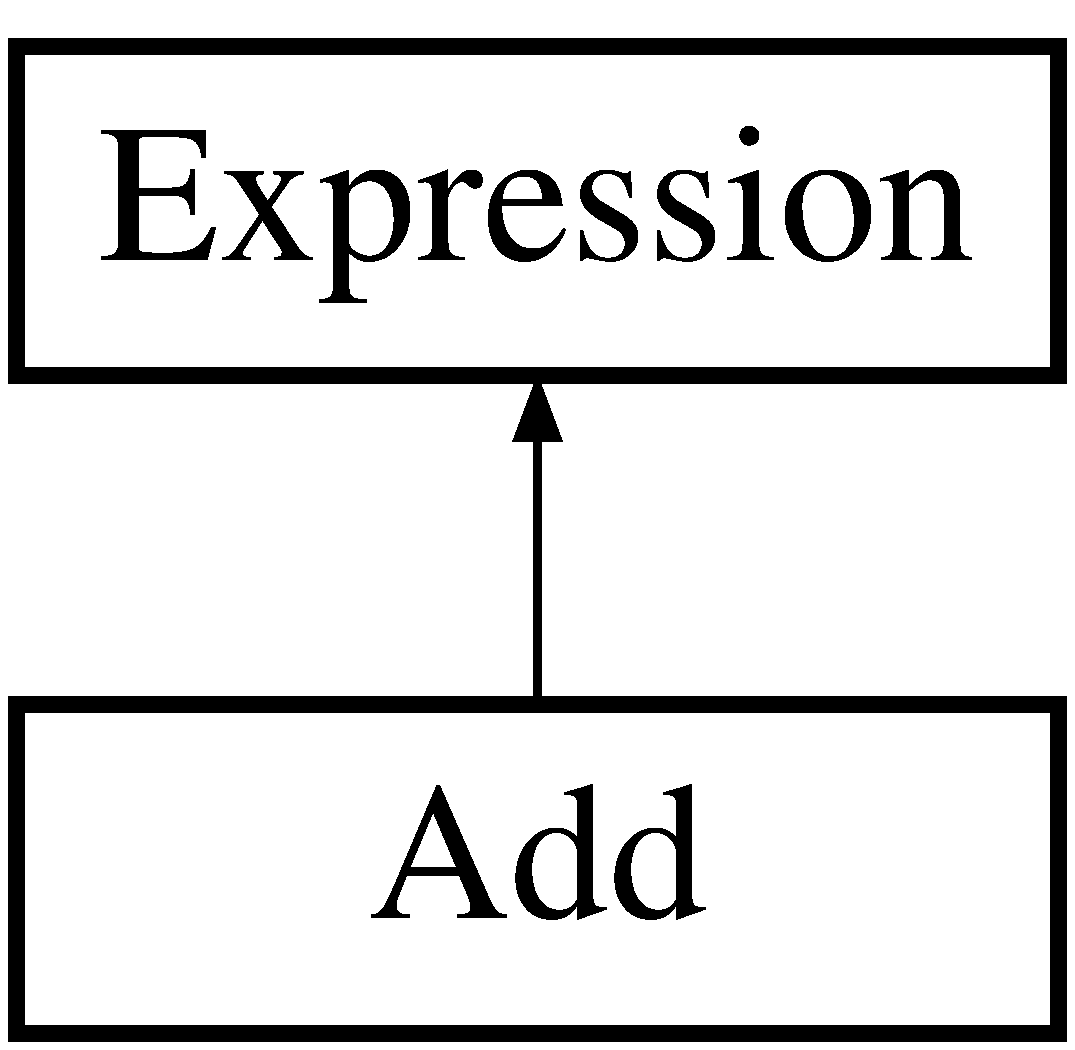
\includegraphics[height=2.000000cm]{class_add}
\end{center}
\end{figure}
\subsection*{Public Member Functions}
\begin{DoxyCompactItemize}
\item 
\mbox{\Hypertarget{class_add_a2e122c2aa72180550626ecded3f26644}\label{class_add_a2e122c2aa72180550626ecded3f26644}} 
{\bfseries Add} (\hyperlink{class_expression}{Expression} $\ast$l, \hyperlink{class_expression}{Expression} $\ast$r)
\item 
\mbox{\Hypertarget{class_add_ac5b3425e7ac47b9f9a83e2f6da0d81ca}\label{class_add_ac5b3425e7ac47b9f9a83e2f6da0d81ca}} 
double {\bfseries evaluate} () const
\item 
\mbox{\Hypertarget{class_add_ad5af4ca57a44efab928c58ef39b00df1}\label{class_add_ad5af4ca57a44efab928c58ef39b00df1}} 
void {\bfseries print} () const
\end{DoxyCompactItemize}


The documentation for this class was generated from the following files\+:\begin{DoxyCompactItemize}
\item 
add.\+h\item 
add.\+cpp\end{DoxyCompactItemize}

\hypertarget{class_const}{}\section{Const Class Reference}
\label{class_const}\index{Const@{Const}}
Inheritance diagram for Const\+:\begin{figure}[H]
\begin{center}
\leavevmode
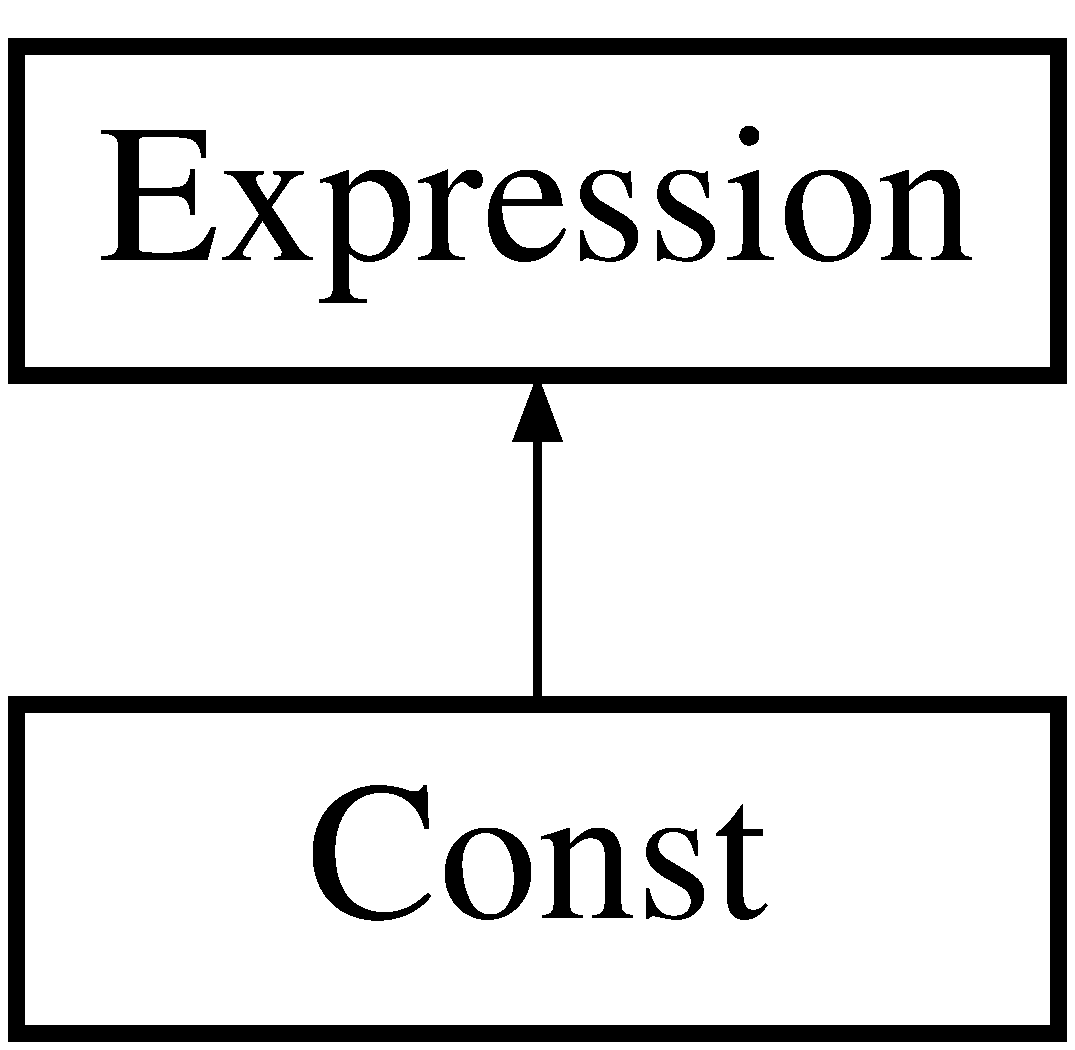
\includegraphics[height=2.000000cm]{class_const}
\end{center}
\end{figure}
\subsection*{Public Member Functions}
\begin{DoxyCompactItemize}
\item 
\mbox{\Hypertarget{class_const_a685dd0971c313a7ccb4a8fd6f3912615}\label{class_const_a685dd0971c313a7ccb4a8fd6f3912615}} 
{\bfseries Const} (double val)
\item 
\mbox{\Hypertarget{class_const_a2f86d9af4cbc9dda466815c66360ba16}\label{class_const_a2f86d9af4cbc9dda466815c66360ba16}} 
double {\bfseries evaluate} () const
\item 
\mbox{\Hypertarget{class_const_a81dc57c45d716e31d1cdb65a2c8f227d}\label{class_const_a81dc57c45d716e31d1cdb65a2c8f227d}} 
void {\bfseries print} () const
\end{DoxyCompactItemize}


The documentation for this class was generated from the following files\+:\begin{DoxyCompactItemize}
\item 
const.\+h\item 
const.\+cpp\end{DoxyCompactItemize}

\hypertarget{class_div}{}\section{Div Class Reference}
\label{class_div}\index{Div@{Div}}
Inheritance diagram for Div\+:\begin{figure}[H]
\begin{center}
\leavevmode
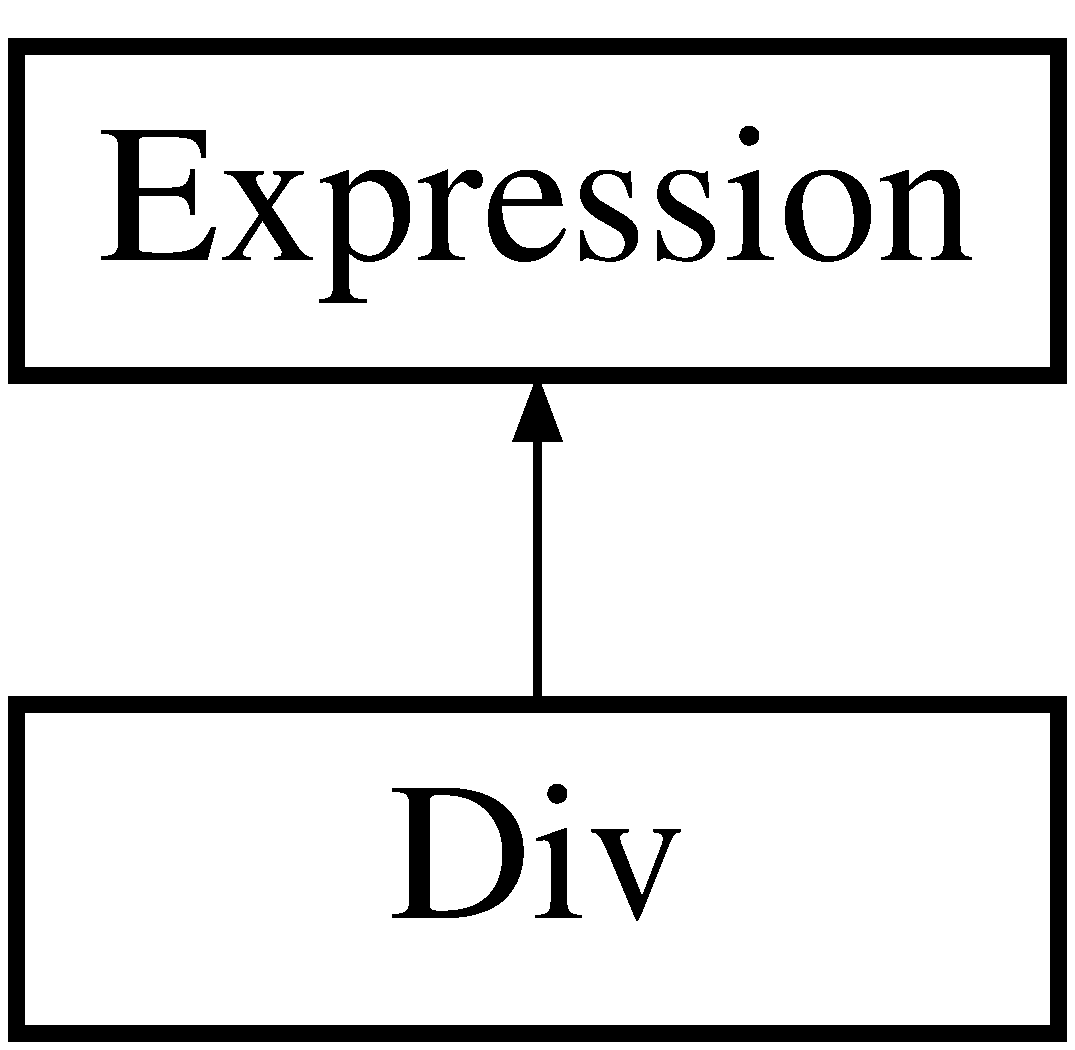
\includegraphics[height=2.000000cm]{class_div}
\end{center}
\end{figure}
\subsection*{Public Member Functions}
\begin{DoxyCompactItemize}
\item 
\mbox{\Hypertarget{class_div_a31f89c83d9d65cf54396ebbea8af809a}\label{class_div_a31f89c83d9d65cf54396ebbea8af809a}} 
{\bfseries Div} (\hyperlink{class_expression}{Expression} $\ast$l, \hyperlink{class_expression}{Expression} $\ast$r)
\item 
\mbox{\Hypertarget{class_div_a5b96e19e7cffdb205a9e56377be3652e}\label{class_div_a5b96e19e7cffdb205a9e56377be3652e}} 
double {\bfseries evaluate} () const
\item 
\mbox{\Hypertarget{class_div_acbcc6e3d0f3ccb5e74de28de8499cbbf}\label{class_div_acbcc6e3d0f3ccb5e74de28de8499cbbf}} 
void {\bfseries print} () const
\end{DoxyCompactItemize}


The documentation for this class was generated from the following files\+:\begin{DoxyCompactItemize}
\item 
div.\+h\item 
div.\+cpp\end{DoxyCompactItemize}

\hypertarget{class_expression}{}\section{Expression Class Reference}
\label{class_expression}\index{Expression@{Expression}}
Inheritance diagram for Expression\+:\begin{figure}[H]
\begin{center}
\leavevmode
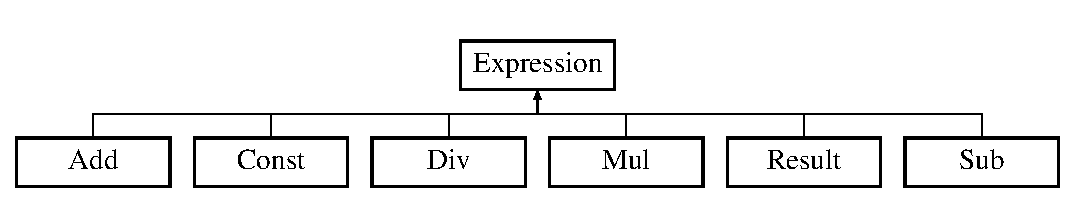
\includegraphics[height=2.000000cm]{class_expression}
\end{center}
\end{figure}
\subsection*{Public Member Functions}
\begin{DoxyCompactItemize}
\item 
\mbox{\Hypertarget{class_expression_a9e2b69592a66b920d052f5e12e1ddb70}\label{class_expression_a9e2b69592a66b920d052f5e12e1ddb70}} 
virtual double {\bfseries evaluate} () const =0
\item 
\mbox{\Hypertarget{class_expression_ae11e78376212134745e5fa9f0b91dbd1}\label{class_expression_ae11e78376212134745e5fa9f0b91dbd1}} 
virtual void {\bfseries print} () const =0
\end{DoxyCompactItemize}


The documentation for this class was generated from the following files\+:\begin{DoxyCompactItemize}
\item 
expression.\+h\item 
expression.\+cpp\end{DoxyCompactItemize}

\hypertarget{class_mul}{}\section{Mul Class Reference}
\label{class_mul}\index{Mul@{Mul}}
Inheritance diagram for Mul\+:\begin{figure}[H]
\begin{center}
\leavevmode
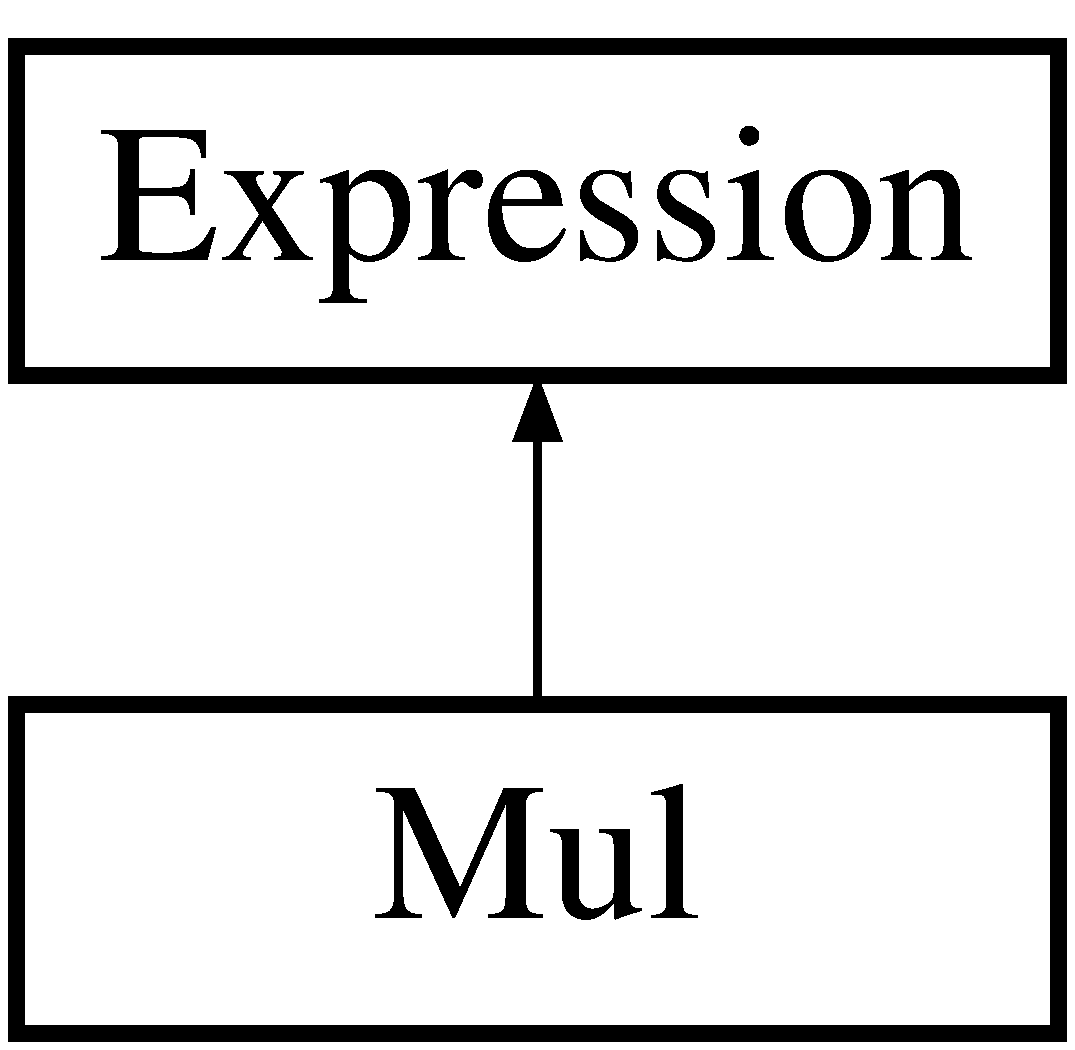
\includegraphics[height=2.000000cm]{class_mul}
\end{center}
\end{figure}
\subsection*{Public Member Functions}
\begin{DoxyCompactItemize}
\item 
\mbox{\Hypertarget{class_mul_a3a22b4fed252912b4795d5d48272e1aa}\label{class_mul_a3a22b4fed252912b4795d5d48272e1aa}} 
{\bfseries Mul} (\hyperlink{class_expression}{Expression} $\ast$l, \hyperlink{class_expression}{Expression} $\ast$r)
\item 
\mbox{\Hypertarget{class_mul_a3e98f760d06aaac61dda9ab57d174a35}\label{class_mul_a3e98f760d06aaac61dda9ab57d174a35}} 
double {\bfseries evaluate} () const
\item 
\mbox{\Hypertarget{class_mul_a0aa9276f2fc04dd9afc77bf47542e5ec}\label{class_mul_a0aa9276f2fc04dd9afc77bf47542e5ec}} 
void {\bfseries print} () const
\end{DoxyCompactItemize}


The documentation for this class was generated from the following files\+:\begin{DoxyCompactItemize}
\item 
mul.\+h\item 
mul.\+cpp\end{DoxyCompactItemize}

\hypertarget{class_result}{}\section{Result Class Reference}
\label{class_result}\index{Result@{Result}}
Inheritance diagram for Result\+:\begin{figure}[H]
\begin{center}
\leavevmode
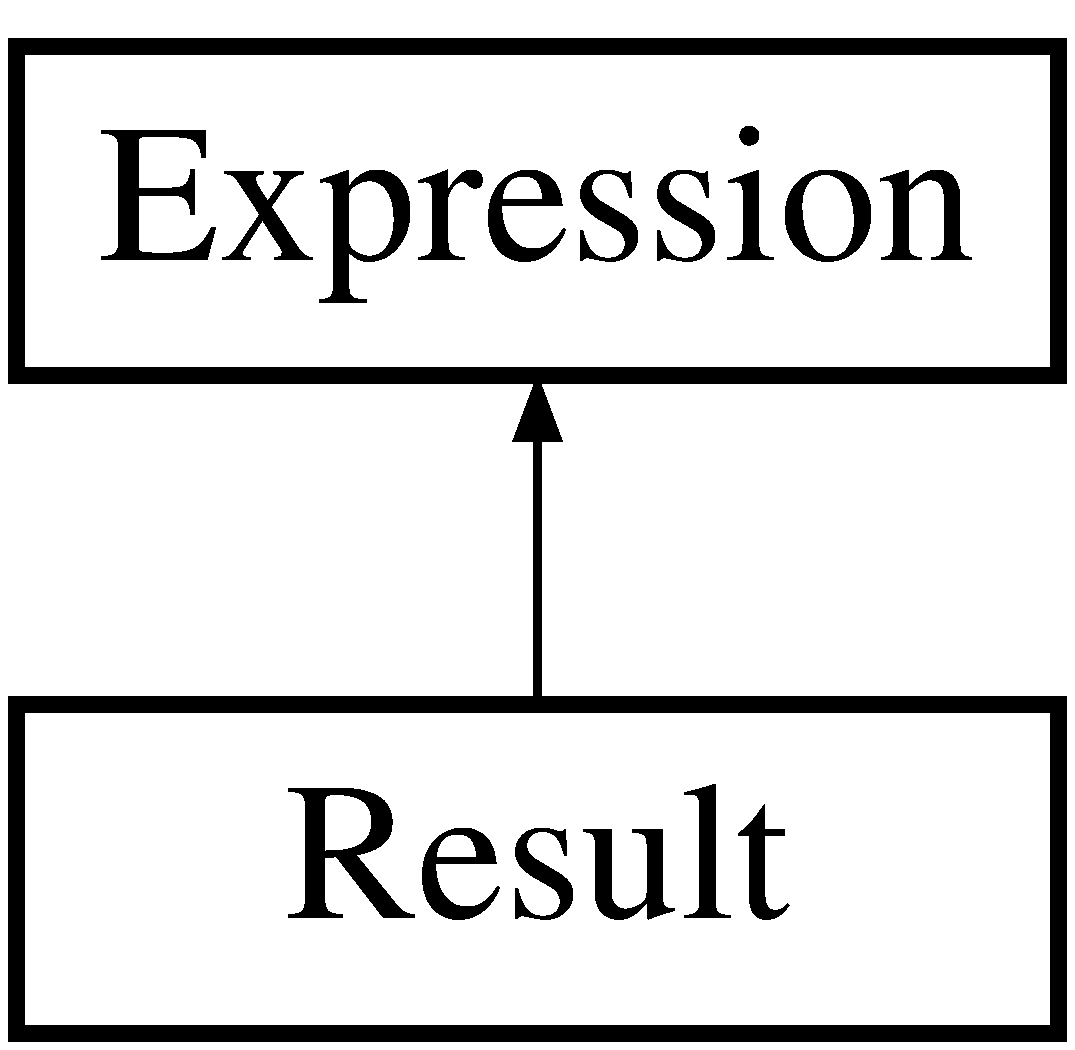
\includegraphics[height=2.000000cm]{class_result}
\end{center}
\end{figure}
\subsection*{Public Member Functions}
\begin{DoxyCompactItemize}
\item 
\mbox{\Hypertarget{class_result_a8fb8868bd4f4e305f436e98e052755f2}\label{class_result_a8fb8868bd4f4e305f436e98e052755f2}} 
{\bfseries Result} (\hyperlink{class_expression}{Expression} $\ast$exp)
\item 
\mbox{\Hypertarget{class_result_a107a060722c095f33008ca435cb2397d}\label{class_result_a107a060722c095f33008ca435cb2397d}} 
double {\bfseries evaluate} () const
\item 
\mbox{\Hypertarget{class_result_a17227de791c97a6eee68689f4317cafa}\label{class_result_a17227de791c97a6eee68689f4317cafa}} 
void {\bfseries print} () const
\end{DoxyCompactItemize}


The documentation for this class was generated from the following files\+:\begin{DoxyCompactItemize}
\item 
result.\+h\item 
result.\+cpp\end{DoxyCompactItemize}

\hypertarget{class_sub}{}\section{Sub Class Reference}
\label{class_sub}\index{Sub@{Sub}}
Inheritance diagram for Sub\+:\begin{figure}[H]
\begin{center}
\leavevmode
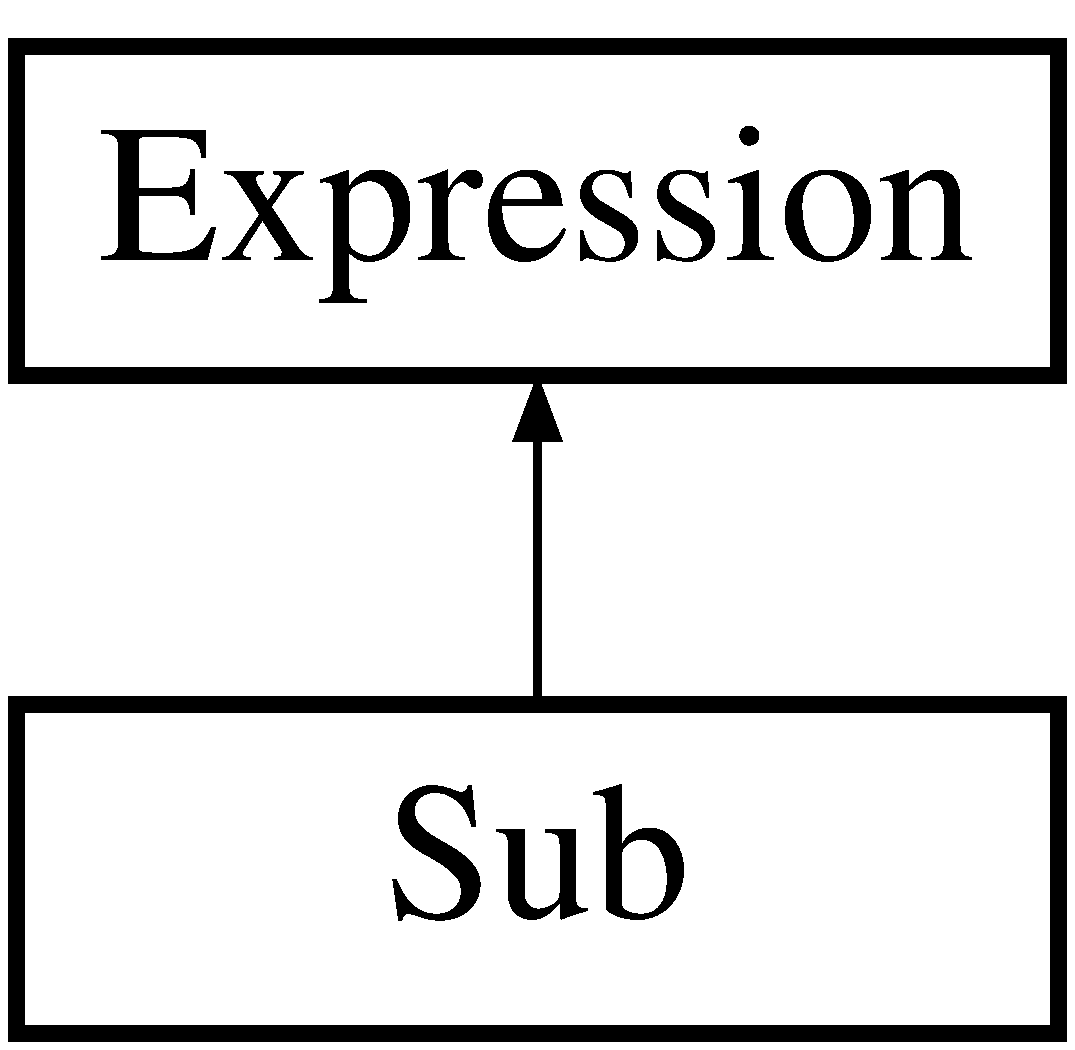
\includegraphics[height=2.000000cm]{class_sub}
\end{center}
\end{figure}
\subsection*{Public Member Functions}
\begin{DoxyCompactItemize}
\item 
\mbox{\Hypertarget{class_sub_a0156785212e8c6b36f9ca03c13ce2f0a}\label{class_sub_a0156785212e8c6b36f9ca03c13ce2f0a}} 
{\bfseries Sub} (\hyperlink{class_expression}{Expression} $\ast$l, \hyperlink{class_expression}{Expression} $\ast$r)
\item 
\mbox{\Hypertarget{class_sub_a15b87b081136f533a993a92ac01ec11b}\label{class_sub_a15b87b081136f533a993a92ac01ec11b}} 
double {\bfseries evaluate} () const
\item 
\mbox{\Hypertarget{class_sub_a2e7c967c1fdee5e7eca51ca36feb26bc}\label{class_sub_a2e7c967c1fdee5e7eca51ca36feb26bc}} 
void {\bfseries print} () const
\end{DoxyCompactItemize}


The documentation for this class was generated from the following files\+:\begin{DoxyCompactItemize}
\item 
sub.\+h\item 
sub.\+cpp\end{DoxyCompactItemize}

%--- End generated contents ---

% Index
\backmatter
\newpage
\phantomsection
\clearemptydoublepage
\addcontentsline{toc}{chapter}{Index}
\printindex

\end{document}
